\documentclass[Royal,times,sageh]{sagej}
%DIF LATEXDIFF DIFFERENCE FILE
%DIF DEL Manuscript-Data-Package_R0.tex   Fri Oct 28 01:12:02 2022
%DIF ADD Manuscript-Data-Package.tex      Fri Oct 28 01:35:46 2022

\usepackage{moreverb,url,natbib, multirow, tabularx}
\usepackage[colorlinks,bookmarksopen,bookmarksnumbered,citecolor=red,urlcolor=red]{hyperref}



% tightlist command for lists without linebreak
\providecommand{\tightlist}{%
  \setlength{\itemsep}{0pt}\setlength{\parskip}{0pt}}



\usepackage{booktabs}
\usepackage{longtable}
\usepackage{array}
\usepackage{multirow}
\usepackage{wrapfig}
\usepackage{float}
\usepackage{colortbl}
\usepackage{pdflscape}
\usepackage{tabu}
\usepackage{threeparttable}
\usepackage{threeparttablex}
\usepackage[normalem]{ulem}
\usepackage{makecell}
\usepackage{xcolor}
%DIF PREAMBLE EXTENSION ADDED BY LATEXDIFF
%DIF UNDERLINE PREAMBLE %DIF PREAMBLE
\RequirePackage[normalem]{ulem} %DIF PREAMBLE
\RequirePackage{color}\definecolor{RED}{rgb}{1,0,0}\definecolor{BLUE}{rgb}{0,0,1} %DIF PREAMBLE
\providecommand{\DIFaddtex}[1]{{\protect\color{blue}\uwave{#1}}} %DIF PREAMBLE
\providecommand{\DIFdeltex}[1]{{\protect\color{red}\sout{#1}}}                      %DIF PREAMBLE
%DIF SAFE PREAMBLE %DIF PREAMBLE
\providecommand{\DIFaddbegin}{} %DIF PREAMBLE
\providecommand{\DIFaddend}{} %DIF PREAMBLE
\providecommand{\DIFdelbegin}{} %DIF PREAMBLE
\providecommand{\DIFdelend}{} %DIF PREAMBLE
\providecommand{\DIFmodbegin}{} %DIF PREAMBLE
\providecommand{\DIFmodend}{} %DIF PREAMBLE
%DIF FLOATSAFE PREAMBLE %DIF PREAMBLE
\providecommand{\DIFaddFL}[1]{\DIFadd{#1}} %DIF PREAMBLE
\providecommand{\DIFdelFL}[1]{\DIFdel{#1}} %DIF PREAMBLE
\providecommand{\DIFaddbeginFL}{} %DIF PREAMBLE
\providecommand{\DIFaddendFL}{} %DIF PREAMBLE
\providecommand{\DIFdelbeginFL}{} %DIF PREAMBLE
\providecommand{\DIFdelendFL}{} %DIF PREAMBLE
%DIF HYPERREF PREAMBLE %DIF PREAMBLE
\providecommand{\DIFadd}[1]{\texorpdfstring{\DIFaddtex{#1}}{#1}} %DIF PREAMBLE
\providecommand{\DIFdel}[1]{\texorpdfstring{\DIFdeltex{#1}}{}} %DIF PREAMBLE
%DIF END PREAMBLE EXTENSION ADDED BY LATEXDIFF

\begin{document}


\setcitestyle{aysep={,}}

\title{TTS2016R: A \DIFdelbegin \DIFdel{dataset }\DIFdelend \DIFaddbegin \DIFadd{data set }\DIFaddend to study population and employment patterns
from the 2016 Transportation Tomorrow Survey (TTS) in the Greater \DIFdelbegin \DIFdel{Toronto and Hamilton }\DIFdelend \DIFaddbegin \DIFadd{Golden
Horseshoe }\DIFaddend Area, \DIFaddbegin \DIFadd{Ontario, }\DIFaddend Canada}

\runninghead{}

\author{\DIFdelbegin \DIFdel{Anastasia Soukhov}\DIFdelend \DIFaddbegin \DIFadd{Anon1}\DIFaddend \affilnum{}, \DIFdelbegin \DIFdel{Antonio Páez}\DIFdelend \DIFaddbegin \DIFadd{Anon2}\DIFaddend \affilnum{}}

\affiliation{\affilnum{}{}}



\begin{abstract}
This paper describes and visualises the data contained within the
\{TTS2016R\} \DIFdelbegin \DIFdel{data-package }\DIFdelend \DIFaddbegin \DIFadd{data package }\DIFaddend created in \texttt{R}, the statistical
computing and graphics language. In addition to a synthetic example,
\{TTS2016R\} contains home-to-work commute information for the Greater
Golden Horseshoe \DIFaddbegin \DIFadd{(GGH) }\DIFaddend area in Canada retrieved from the 2016
Transportation Tomorrow Survey (TTS). Included are all Traffic Analysis
Zones (TAZ), the number of people who are employed full-time per TAZ,
the number of jobs per TAZ, \DIFdelbegin \DIFdel{origin-destination trips , and }\DIFdelend \DIFaddbegin \DIFadd{the count of origin destination (OD) pairs
and trips by mode per origin TAZ, }\DIFaddend calculated car travel time from TAZ \DIFdelbegin \DIFdel{origin-destination centroid pairs}\DIFdelend \DIFaddbegin \DIFadd{OD
centroid pairs, and associated spatial boundaries to link TAZ to the
Canadian Census}\DIFaddend . To illustrate how this information can be analysed to
understand patterns in commuting, we estimate a distance-decay curve
(i.e., impedance function) for the region. \{TTS2016R\} \DIFaddbegin \DIFadd{is a growing
open data product built on }\texttt{\DIFadd{R}} \DIFadd{infrastructure that allows for the
immediate access of home-to-work commuting data alongside complimentary
objects from different sources. The package will continue expanding with
additions by the authors and the community at-large by requests in the
future. \{TTS2016R\} }\DIFaddend can be freely \DIFdelbegin \DIFdel{downloaded and explored at:
}%DIFDELCMD < \url{https://github.com/soukhova/TTS2016R} %%%
\DIFdelend \DIFaddbegin \DIFadd{explored and downloaded in the
associated }\href{https://github.com/soukhova/TTS2016R}{\DIFadd{Github
repository}} \DIFaddend where the documentation and code involved in data creation,
manipulation, and \DIFdelbegin \DIFdel{the final }\DIFdelend \DIFaddbegin \DIFadd{all open }\DIFaddend data products are detailed.
\end{abstract}

\DIFdelbegin %DIFDELCMD < \keywords{Jobs; population; travel time; impedance; Greater Toronto and
%DIFDELCMD < Hamilton Area; Ontario, Canada; R}
%DIFDELCMD < %%%
\DIFdelend \DIFaddbegin \keywords{Jobs; population; work; commute; travel time; impedance;
Greater Toronto and Hamilton Area; Greater Golden Horshoe Area, Ontario,
Canada; R}
\DIFaddend 

\maketitle

\hypertarget{introduction}{%
\section{Introduction}\label{introduction}}

This manuscript presents the open data product
\href{https://github.com/soukhova/TTS2016R}{\{TTS2016R\}}. Open data
products are the result of turning source data (open or otherwise) into
accessible information that adds value to the original inputs
\citep[see][]{Arribas2021open}. The product presented in this paper is \DIFdelbegin \DIFdel{an }\DIFdelend \DIFaddbegin \DIFadd{a
}\DIFaddend \texttt{R} data package which currently consists of \DIFdelbegin \DIFdel{three objects
which are }\DIFdelend \DIFaddbegin \DIFadd{a fusion of objects
from a variety of sources: home-to-work flows }\DIFaddend sourced from the 2016
Transportation Tomorrow Survey (TTS)
\DIFdelbegin \DIFdel{or
are curated to facilitate the use and analysis of TTS data.
This packageincludes person-to-jobs origin-destinations}\DIFdelend \DIFaddbegin \DIFadd{\mbox{%DIFAUXCMD
\citep{data_management_group_tts_2018}}\hskip0pt%DIFAUXCMD
, estimated travel times
(calculated using \{r5r\} \mbox{%DIFAUXCMD
\citep{Pereira2021r5r}}\hskip0pt%DIFAUXCMD
), and boundary files
from the TTS \mbox{%DIFAUXCMD
\citep{datamanagementgroupSurveyBoundaryFiles2018} }\hskip0pt%DIFAUXCMD
and from
the Canadian Census \mbox{%DIFAUXCMD
\citep{statisticscanadaBoundaryFiles20162017}}\hskip0pt%DIFAUXCMD
.
}

\DIFadd{What is a }\texttt{\DIFadd{R}} \DIFadd{data package? A }\texttt{\DIFadd{R}} \DIFadd{data package contains
code, data, and documentation in a standardised collection format that
can be installed by }\texttt{\DIFadd{R}} \DIFadd{users through a centralized software
repository such as CRAN (the Comprehensive R Archive Network) and
GitHub. \{TTS2016R\} is freely available on GitHub for all to install
and freely use in the spirit of open and reproducible research.
Currently and in more detail, \{TTS2016R\} includes full-time home-based
work-to-job origin destinations (OD) counts and mode-specific trip
numbers retrieved from the 2016 TTS}\DIFaddend , traffic analysis zone (TAZ)
boundaries, and \DIFdelbegin \DIFdel{planning/municipality}\DIFdelend \DIFaddbegin \DIFadd{municipality, planning, and census metropolitan area
}\DIFaddend boundaries for the Greater Golden Horse area (GGH) located in southern
Ontario, Canada\DIFdelbegin \DIFdel{\mbox{%DIFAUXCMD
\citep{data_management_group_tts_2018}}\hskip0pt%DIFAUXCMD
}\DIFdelend . In addition, the package includes TAZ
centroid-to-centroid travel times by car\DIFaddbegin \DIFadd{, transit, cycling, and walking
mode }\DIFaddend computed using package \{r5r\} \citep{Pereira2021r5r}.
\DIFaddbegin 

\DIFaddend The aim of this paper is to walk readers through the \DIFdelbegin \DIFdel{empirical home-based work commute data set,
illustrate }\DIFdelend \DIFaddbegin \DIFadd{data sets,
illustrate a use case (i.e., }\DIFaddend the calculation of an impedance function
that can be used to calculate accessibility to employment\DIFaddbegin \DIFadd{)}\DIFaddend , and invite
\DIFdelbegin \DIFdel{its use in other
applications. }\DIFdelend \DIFaddbegin \DIFadd{others to experiment in its uses and applications. Though data from the
TTS is freely available to the public through the
}\href{https://dmg.utoronto.ca/idrs/index}{\DIFadd{TTS Data Retrieval System}}\DIFadd{,
the raw data can be technically demanding, cumbersome to work with, and
requires multiple software to process. By pre-processing the data,
packaging it with complimentary data, and providing explicit
documentation in a }\texttt{\DIFadd{R}} \DIFadd{environment, \{TTS2016R\} offers a slice
of the TTS data that can be immediately used by }\texttt{\DIFadd{R}} \DIFadd{users to
analysis patterns of commuting to work in the region. Anticipate this
package to grow in the future: it currently provides an open
infrastructure for additional TTS or complimentary data sets to be
amended by the authors and the open-source community in the future by
request.
}\DIFaddend 

\hypertarget{home-to-work-commute-data}{%
\section{Home-to-work commute data}\label{home-to-work-commute-data}}

\DIFaddbegin \DIFadd{Currently, }\DIFaddend \{TTS2016R\} includes counts of \DIFdelbegin \DIFdel{fully-employed }\DIFdelend \DIFaddbegin \DIFadd{full-time employed }\DIFaddend population
by place of residence (origin)\DIFdelbegin \DIFdel{and }\DIFdelend \DIFaddbegin \DIFadd{, }\DIFaddend counts of full-time \DIFdelbegin \DIFdel{jobs by }\DIFdelend \DIFaddbegin \DIFadd{usual }\DIFaddend place of work
(destination)\DIFdelbegin \DIFdel{aggregated by TAZ (n=3, 764 within the survey boundaries) .
TAZ typically are defined based on land-use and population demographics
in order }\DIFdelend \DIFaddbegin \DIFadd{, number of trips to work by mode, and the calculated
potential travel time of the trips in the GGH. The GGH (and hence the
TTS survey area) is displayed in Figure \ref{fig:TTS-16-survey-area}.
}

\DIFadd{This data is aggregated and available at the level of TAZ: TAZ are a
spatial unit of analysis typically used }\DIFaddend to estimate the number of trips
produced and attracted to each zone \citep{meyer_urban_2001}. \DIFdelbegin \DIFdel{As such, }\DIFdelend \DIFaddbegin \DIFadd{They are
thus defined by transportation planners for a region based on
intra-similarity and inter-dissimilarity between land-use and population
demographics. Within the GGH boundaries, 3,764 TAZ are specified and
}\DIFaddend each TAZ is uniquely identified using the GTA06 Zoning System\DIFdelbegin \DIFdel{which can be used to join to the
origin-destination table (i.e., trips taken).
}%DIFDELCMD < 

%DIFDELCMD < %%%
\DIFdel{The number of jobs (3,081,885) and workers (3,446,957) in this package
are organized in the form of an origin-destination table which is
indicative of home-to-work commute patterns (there are 3,446,957
potential interactions). These data were retrieved from the TTS Data
Retrieval System on October 28, 2021 and reflect the potential
interaction of full-time employed people and jobs within the GGH survey
boundaries shown in Figure \ref{fig:TTS-16-survey-area} as }\DIFdelend \DIFaddbegin \DIFadd{: the
survey boundary is discussed in the 2016 TTS methodology and }\DIFaddend defined by
the \DIFdelbegin \DIFdel{2016 TTS methodology \mbox{%DIFAUXCMD
\citep{data_management_group_tts_2018}}\hskip0pt%DIFAUXCMD
. }%DIFDELCMD < 

%DIFDELCMD < %%%
\DIFdel{Also included in \{TTS2016R\} are travel times and cost of travel from
origin to destination by car; travel times are calculated using the
}\texttt{\DIFdel{R}} %DIFAUXCMD
\DIFdel{package \{r5r\}. These travel times are useful to estimate
the cost of travel and to calculate impedance functions, among other
possible applications. For simplicity, all interactions within
\{TTS2016R\} are assumed to be taken by car, and the travel time is
calculated from an origin TAZ centroid to a destination TAZ centroid.
The centroid is snapped to the nearest street line by }\texttt{\DIFdel{r5r}} %DIFAUXCMD
\DIFdel{and
the travel time is calculated for all trips assuming a car travel mode.
Additionally, only travel times less than or equal to 180 mins (3 hrs)are calculated; this threshold represents 99\% of trip's travel times
which are summarized in Figure \ref{fig:TTS-16-survey-area}}\DIFdelend \DIFaddbegin \DIFadd{TTS \mbox{%DIFAUXCMD
\citep{data_management_group_tts_2018}}\hskip0pt%DIFAUXCMD
}\DIFaddend . \DIFaddbegin \DIFadd{The TAZ range between
\(\ge\) 0.019 km\textsuperscript{2} in spatial area to a maximum of 879
km\textsuperscript{2} (median: 1.3 km\textsuperscript{2} and 3rd
quantile: 2.8 km\textsuperscript{2}).
}\DIFaddend 

\begin{figure}[H]

{\centering 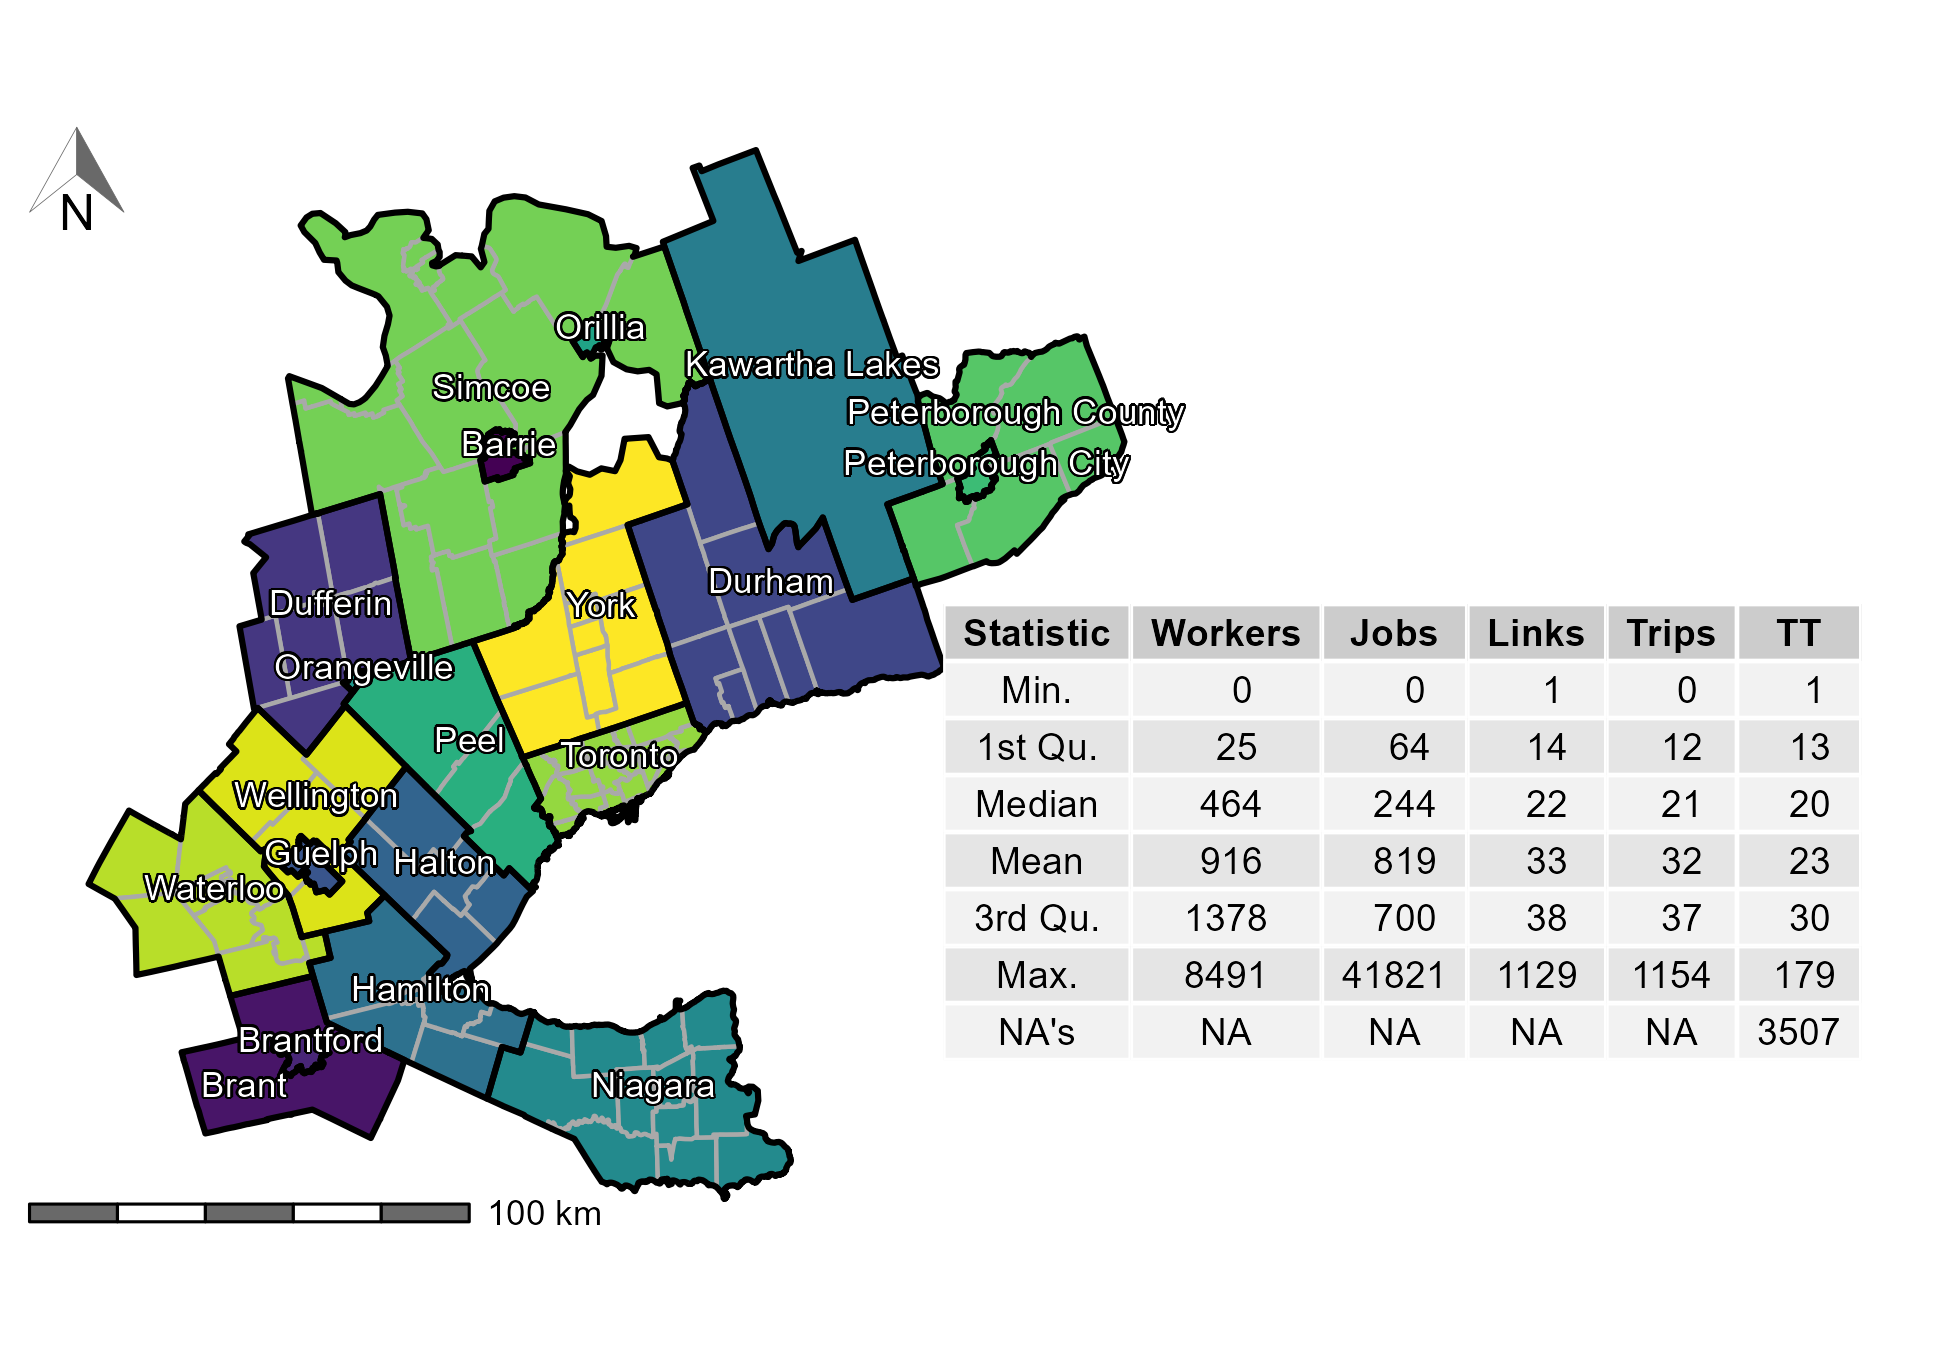
\includegraphics[width=1\linewidth]{images/TTS16-survey-area} 

}

\caption{\label{fig:TTS-16-survey-area}TTS 2016 study area within the GGH in Ontario, Canada along with \DIFdelbeginFL \DIFdelFL{the }\DIFdelendFL \DIFaddbeginFL \DIFaddFL{associated }\DIFaddendFL descriptive \DIFdelbeginFL \DIFdelFL{statistics }\DIFdelendFL \DIFaddbeginFL \DIFaddFL{statistic }\DIFaddendFL of \DIFdelbeginFL \DIFdelFL{the trips}\DIFdelendFL \DIFaddbeginFL \DIFaddFL{workers and jobs per TAZ}\DIFaddendFL , \DIFaddbeginFL \DIFaddFL{OD links (count of workers potentially interacting with their place of employment) by origin TAZ, and }\DIFaddendFL calculated \DIFdelbeginFL \DIFdelFL{origin-destination }\DIFdelendFL \DIFaddbeginFL \DIFaddFL{OD }\DIFaddendFL car travel time (TT) \DIFdelbeginFL \DIFdelFL{, workers }\DIFdelendFL per \DIFaddbeginFL \DIFaddFL{origin }\DIFaddendFL TAZ\DIFaddbeginFL \DIFaddFL{. 3}\DIFaddendFL ,\DIFdelbeginFL \DIFdelFL{and jobs per TAZ}\DIFdelendFL \DIFaddbeginFL \DIFaddFL{507 trips were not assigned TT as they are longer than 180 mins}\DIFaddendFL . \DIFdelbeginFL \DIFdelFL{Contains }\DIFdelendFL \DIFaddbeginFL \DIFaddFL{Spatial boundary files are retrieved from the TTS which define the survey area (Data Management Group, 2018a): the }\DIFaddendFL 20 regions \DIFdelbeginFL \DIFdelFL{(}\DIFdelendFL \DIFaddbeginFL \DIFaddFL{in the GGH are represented by }\DIFaddendFL black \DIFdelbeginFL \DIFdelFL{boundaries) }\DIFdelendFL \DIFaddbeginFL \DIFaddFL{lines }\DIFaddendFL and \DIFdelbeginFL \DIFdelFL{sub-regions (}\DIFdelendFL \DIFaddbeginFL \DIFaddFL{labelled, the }\DIFaddendFL dark gray \DIFaddbeginFL \DIFaddFL{lines are planning }\DIFaddendFL boundaries\DIFdelbeginFL \DIFdelFL{)}\DIFdelendFL .}\label{fig:TTS-16-survey-area}
\end{figure}

\DIFdelbegin %DIFDELCMD < \hypertarget{employed-individuals-and-jobs}{%
%DIFDELCMD < \subsection{Employed individuals and
%DIFDELCMD < jobs}\label{employed-individuals-and-jobs}}
%DIFDELCMD < %%%
\DIFdelend \DIFaddbegin \hypertarget{full-time-employed-people-and-associated-places-of-employment}{%
\subsection{Full-time employed people and associated places of
employment}\label{full-time-employed-people-and-associated-places-of-employment}}
\DIFaddend 

\DIFdelbegin \DIFdel{The origin-destination table (i.e., trips) consists of a
}\DIFdelend \DIFaddbegin \DIFadd{In the GGH, there are 3,446,957 workers, 3,081,900 jobs, and 3,282,611
work-related trips (for the 2016 TTS survey day). The values are
organized within the origin destination (OD) table in the \{TTS2016R\}
package and are derived from the }\DIFaddend cross-tabulation \DIFdelbegin \DIFdel{of people who are
employed }\DIFdelend \DIFaddbegin \DIFadd{by person and by trip
for the }\DIFaddend full-time \DIFdelbegin \DIFdel{by place of GGH
residence (origin ) and places of GGH employment(destination) using the
GTA06 TAZ zoning system.
It is important to note that }\DIFdelend \DIFaddbegin \DIFadd{employed population and associated places of
employment.
}

\DIFadd{Additionally, }\DIFaddend the total number of \DIFaddbegin \DIFadd{full-time }\DIFaddend workers and jobs \DIFdelbegin \DIFdel{is }\DIFdelend \DIFaddbegin \DIFadd{in }\DIFaddend the TTS
2016 region are not equal\DIFdelbegin \DIFdel{but the number
of trips taken are equal to the number of workers}\DIFdelend . Since the outer boundaries of the TTS are
permeable, workers who reside within the boundaries but \DIFdelbegin \DIFdel{travel }\DIFdelend \DIFaddbegin \DIFadd{have workplaces
that are }\DIFaddend outside of the boundaries are counted as workers within an
origin TAZ, while jobs in TAZ that are filled by workers who reside
outside the GGH boundaries are \emph{unknown} since they were not
surveyed. This mismatch results in the total number of workers being
1.12 times larger than the number of jobs\DIFdelbegin \DIFdel{(i. e., 3,446,957 workers to
3,081,885 jobs). As such, the origin-destination table contained }\DIFdelend \DIFaddbegin \DIFadd{. The TTS is a proportionally
representative survey, hence the values included }\DIFaddend in \{TTS2016R\} \DIFdelbegin \DIFdel{offers a perspective on all workers in the GGH }\DIFdelend \DIFaddbegin \DIFadd{are
adjusted to reflect the GGH working population }\DIFaddend and their home-based
trips to places of GGH employment.

\DIFaddbegin \DIFadd{The count of links and trips made by the full-time working population
and associated full-time place of employment per unique OD pair are
quite variable. TAZ contain between 0 to 8,491 workers (median: 464, 3rd
quantile: 1,378), 0 to 41,821 jobs (median: 244, 3rd quantile: 700), and
generate between 0 to 241 trips (median: 15, 3rd quantile: 42).
}

\DIFaddend \begin{figure}
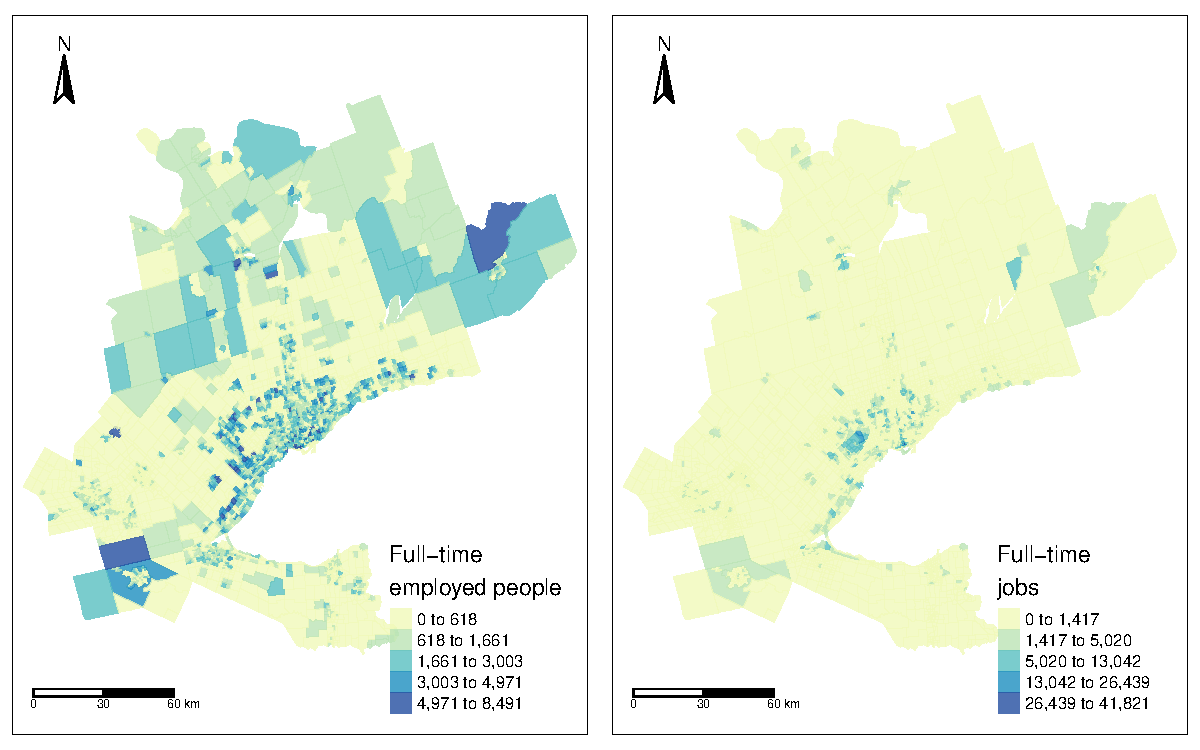
\includegraphics[width=1\linewidth]{Manuscript-Data-Package_files/figure-latex/tts-workers-jobs-plot-1} \caption{\label{fig:tts-workers-jobs-plot}Number of workers (left) and jobs (right) in each TAZ \DIFdelbeginFL \DIFdelFL{in }\DIFdelendFL \DIFaddbeginFL \DIFaddFL{retrieved from }\DIFaddendFL the 2016 TTS \DIFaddbeginFL \DIFaddFL{(Data Management Group, 2018b)}\DIFaddendFL . \DIFaddbeginFL \DIFaddFL{Spatial boundary files are retrieved from the TAZ defined by the TTS (Data Management Group, 2018a).}\DIFaddendFL }\label{fig:tts-workers-jobs-plot}
\end{figure}

Figure \ref{fig:tts-workers-jobs-plot} presents the number of \DIFdelbegin \DIFdel{workers
and }\DIFdelend \DIFaddbegin \DIFadd{employed
people and associated }\DIFaddend jobs per TAZ. It can be observed that the spatial
distribution of jobs and workers is unequal, which is indicative of a
\DIFdelbegin \DIFdel{jobs-housing
}\DIFdelend \DIFaddbegin \DIFadd{jobs -housing }\DIFaddend imbalance that can impact accessibility in a region
\citep{Levine1998rethinking}. \DIFdelbegin \DIFdel{It can also be seen that }\DIFdelend \DIFaddbegin \DIFadd{Also, }\DIFaddend there is a higher number of TAZ with
no workers than zones with no jobs (i.e., 791 TAZ with no workers \DIFdelbegin \DIFdel{: }\DIFdelend \DIFaddbegin \DIFadd{and
}\DIFaddend 396 TAZ with no jobs) and the mean of workers per TAZ is higher than the
mean of jobs\DIFdelbegin \DIFdel{(i. e., 916 workers : 819 jobs) the
}\DIFdelend \DIFaddbegin \DIFadd{. The }\DIFaddend number TAZ with an extreme number of jobs at the
highest and lowest percentiles is significantly higher than the number
of workers.

\hypertarget{calculated-travel-time}{%
\subsection{Calculated travel time}\label{calculated-travel-time}}

\DIFdelbegin \DIFdel{As mentioned, }\DIFdelend \DIFaddbegin \DIFadd{Also included in }\DIFaddend \{TTS2016R\} \DIFdelbegin \DIFdel{also includes travel time data for each
home-to-work trip as displayed in Figure \ref{fig:plot-tt-ttpertrip}.
This travel time corresponds to a car commute }\DIFdelend \DIFaddbegin \DIFadd{are the estimated travel times between OD
as summarized in the descriptive statistics table in Figure
\ref{fig:plot-tt-ttpertrip}; travel times are }\DIFaddend calculated using the
\DIFdelbegin \DIFdel{R
}\DIFdelend package \{r5r\}\DIFdelbegin \DIFdel{(see descriptive statistics in Figure
\ref{fig:TTS-16-survey-area}). It is important to note that travel times
within this
data set are calculated assuming only car travel and one
departure time for all origins. These assumptions are not completely
realistic since we know a small proportion of
trips are taken by non-car
modes and travel }\DIFdelend \DIFaddbegin \DIFadd{. \{r5r\} interfaces with the java-based R5 routing
engine developed separately by Conveyal
\mbox{%DIFAUXCMD
\citep{conveyalConveyalR5Routing2022}}\hskip0pt%DIFAUXCMD
. The inputs to \{r5r\} for this
data package were: the desired mode, a maximum travel }\DIFaddend time \DIFdelbegin \DIFdel{departures varies.
However, it is not possible
from the data retrieval system to obtain higher order tabulations so we
carry on with the assume that all }\DIFdelend \DIFaddbegin \DIFadd{threshold of
180 minutes, the geo-coded origin destination pairs based on the
centroids of the TAZ, and the static OpenStreetMap road network of
Ontario (retrieved using Geofabrick
\mbox{%DIFAUXCMD
\citep{geofabrikOntarioOpenStreetMapGeofabrik2022}}\hskip0pt%DIFAUXCMD
). A travel time
threshold of 180 minutes was selected since it captures almost all
potential OD interactions.
}

\DIFadd{Additionally, car travel is included in this data package because it is
a critically important commute mode in the GGH. 2,598,379 of the trips
are made using a car out of the total 3,282,611 work-related trips
according to the TTS 2016 data (i.e., 79\% of }\DIFaddend trips are taken by \DIFdelbegin \DIFdel{one-time departure
cartrip}\DIFdelend \DIFaddbegin \DIFadd{car)}\DIFaddend .

\DIFaddbegin \DIFadd{These travel times are a useful addition to \{TTS2016R\} since they are
not included in the }\href{https://dmg.utoronto.ca/idrs/index}{\DIFadd{TTS Data
Retrieval System}} \DIFadd{but they are vitally important to estimate the cost of
travel and associated impedance functions, among other possible
applications. If the readership is interested in additional information
regarding the travel time computation, please see the calculation
notebook in the documentation of \{TTS2016R\} and details about \{r5r\}
at the }\href{https://ipeagit.github.io/r5r/index.html}{\DIFadd{r5r package
website}}\DIFadd{.
}

\DIFaddend \begin{figure}
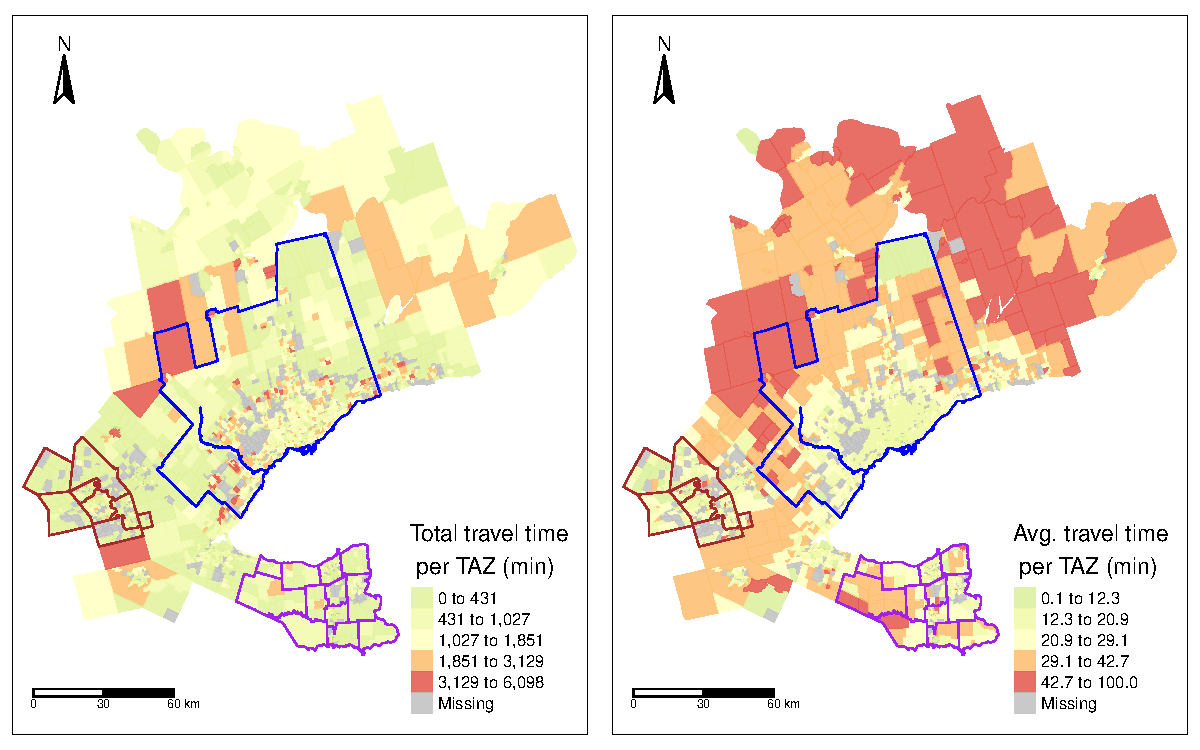
\includegraphics[width=1\linewidth]{Manuscript-Data-Package_files/figure-latex/plot-tt-ttpertrip-1} \caption{\label{fig:plot-tt-ttpertrip}Calculated total worker travel time \DIFaddbeginFL \DIFaddFL{by car }\DIFaddendFL (left) and average worker travel time \DIFaddbeginFL \DIFaddFL{by car }\DIFaddendFL (right) for each TAZ in the 2016 TTS. \DIFaddbeginFL \DIFaddFL{Car travel times calculated using }{\DIFaddFL{r5r}} \DIFaddFL{(Pereira et al., 2021). Planning boundaries of Niagara and Waterloo (Data Management Group, 2018a), and the Toronto census metropolitan area (Statistics Canada, 2017) are drawn with purple, brown and blue borders, respectively. }\DIFaddendFL }\label{fig:plot-tt-ttpertrip}
\end{figure}
\newpage

As can be observed in Figure \ref{fig:plot-tt-ttpertrip}, the total
travel time resembles the spatial trend distribution in the number of
employed people in the previous plot (Figure
\ref{fig:tts-workers-jobs-plot}) and the spatial distribution of the
average travel time is distinct from other plots presented so far. \DIFdelbegin \DIFdel{We
}\DIFdelend \DIFaddbegin \DIFadd{For
instance, we }\DIFaddend can see that in areas around the south-eastern border \DIFdelbegin \DIFdel{that make up the
Greater Toronto and Hamilton Area (GTHA), Niagara and Waterloo, }\DIFdelend \DIFaddbegin \DIFadd{such
as Niagara and Waterloo (purple and brown borders), }\DIFaddend the average travel
times are moderately low. \DIFaddbegin \DIFadd{Additionally, travel times (by car) within the
core of the Toronto census metropolitan area (CMA) (blue) is also
moderately low since traffic congestion is not reflected in the travel
time calculations. }\DIFaddend Further from these areas, travel times are higher.
\DIFdelbegin \DIFdel{Interestingly, even in eastern areas (e.g.,
Peterborough) with high employment and high job concentration, average
travel time is higher than within the GTHA.
}\DIFdelend 

\hypertarget{calibrating-an-impedance-function}{%
\subsection{Calibrating an impedance
function}\label{calibrating-an-impedance-function}}

\DIFaddbegin \DIFadd{An application of the \{TTS2016R\} package is the calculation of an
impedance function. }\DIFaddend Impedance functions are useful to understand
mobility behaviour and are used to estimate gravity models of spatial
interaction \citep{wilson1971, haynes_gravity_1985} and applied in
accessibility analysis
\citep{hansen_how_1959, talen_assessing_1998, paez_jobs_2013, barboza_balancing_2021}.
An impedance function \(f(\cdot)\) depends on the cost of travel
\(c_{ij}\) between locations \(i\) and \(j\) (all which is supplied in
the travel time and origin-destination table within \{TTS2016R\}).

A useful technique to calibrate an impedance function is to use the trip
length distribution (TLD) as measured from origin-destination data
\citep{horbachov_theoretical_2018, batista_estimation_2019}. The TLD is
the representation of the likelihood that a proportion of trips are
taken at a specific travel cost. In our data set, where we assume cost
is travel time, the impedance function maps low travel times to higher
proportions of trips, and high travel times are mapped to low proportion
of trips.

Using the data contained in \{TTS2016R\}, we fit the empirical TLD to a
density distribution using maximum likelihood techniques and the
Nelder-Mead method for direct optimization available within the
\texttt{R} package \{fitdistrplus\} \citep{fitdistrplus_2015}. Based on
goodness-of-fit criteria and diagnostics seen in Figure
\ref{fig:TLD-Gamma-plot}, the gamma distribution is selected. The
`shape' parameter is \(\alpha\) = 2.019, the estimated `rate' is
\(\beta\) = 0.094 , and \(\Gamma(\alpha)\) is defined in Equation
(\ref{gamma-dist}).

\begin{figure}

{\centering 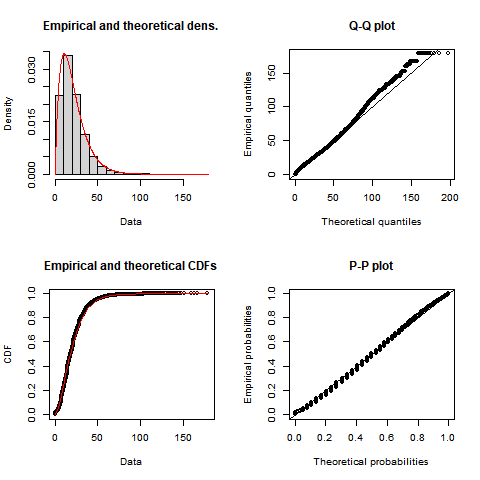
\includegraphics[width=0.75\linewidth]{images/impedance_function} 

}

\caption{\label{fig:TLD-Gamma-plot}Empirical TTS 2016 home-based car TLD (black) and calibrated gamma distribution impedance function (red) with associated Q-Q and P-P plots}\label{fig:TLD-Gamma-plot}
\end{figure}

\DIFdelbegin %DIFDELCMD < \renewcommand{\[\]{\begin{equation}}
%DIFDELCMD < \renewcommand{}}{\end{equation}}
%DIFDELCMD < 

%DIFDELCMD < %%%
\[
\DIFdel{\begin{aligned}
f(x, \alpha, \beta) = \frac{x^{\alpha-1}e^{-\frac{x}{\beta}}}{ \beta^{\alpha}\Gamma(\alpha)} \quad \text{for } 0 \leq x \leq \infty %DIFDELCMD < \label{gamma-dist} %%%
\\
\Gamma(\alpha) =  \int_{0}^{\infty} x^{\alpha-1}e^{-x} \,dx
\end{aligned}
}\]%DIFAUXCMD
\DIFdelend \DIFaddbegin \begin{equation}
\DIFadd{\label{gamma-dist}
\begin{array}{l}\ 
f(x, \alpha, \beta) = \frac{x^{\alpha-1}e^{-\frac{x}{\beta}}}{ \beta^{\alpha}\Gamma(\alpha)} \quad \text{for } 0 \leq x \leq \infty\\
\Gamma(\alpha) =  \int_{0}^{\infty} x^{\alpha-1}e^{-x} \,dx\\
\end{array}
}\end{equation}\DIFaddend 

\DIFaddbegin \newpage
\DIFdelend \hypertarget{concluding-remarks}{%
\section{Concluding remarks}\label{concluding-remarks}}

\DIFdelbegin \DIFdel{The }\DIFdelend \DIFaddbegin \DIFadd{This paper introduces \{TTS2016R\}, an }\DIFaddend open data product \DIFdelbegin \DIFdel{introduced in this paper shares tables }\DIFdelend \DIFaddbegin \DIFadd{in the form of
a }\texttt{\DIFadd{R}} \DIFadd{data package. This package is a fusion of data from
multiple sources and we demonstrate the spatial and numeric extent of
the data contained within. It includes an OD cross-tabulation by person
and by trip mode table }\DIFaddend for home-to-work \DIFdelbegin \DIFdel{related }\DIFdelend \DIFaddbegin \DIFadd{commute }\DIFaddend data from the 2016 TTS
\DIFdelbegin \DIFdel{. In addition, inter-centroid
travel time tables are calculated, and the planning/municipality
boundaries are included as a compliment. This open data product,
\{TTS2016R\}, is freely available to explore in an }\DIFdelend \DIFaddbegin \DIFadd{alongside complimentary boundaries and estimated travel times. The value
of this data package is in its transparency, easy of access, and its
open infrastructure for the addition of complimentary data sets in the
future. }\DIFaddend \texttt{R} \DIFdelbegin \DIFdel{environment}\DIFdelend \DIFaddbegin \DIFadd{users can immediately and easily explore GGH commute
flow trends as well as suggestion further amendments to the package by
request}\DIFaddend . One possible use of this data, as showcased in this paper, is
the calibration of impedance functions which in turn can be used for
accessibility analysis.

In the spirit of novel and original research, we hope readers value the
efforts made to detail the data in order to improve transparency in our
work and encourage others to replicate and, hopefully, inspire research
of their own. We see this product as providing open infrastructure for
additional TTS or complimentary data sets to be amended by the authors
or wider open-source community in the future.

\bibliographystyle{sageh}
\bibliography{bibfile.bib}


\end{document}
